\documentclass[a4paper,11pt]{article}

\usepackage[utf8]{inputenc}
\usepackage[T1]{fontenc}
\usepackage[french]{babel}
\usepackage{graphicx}
\graphicspath{{images/}}
\usepackage{listings}

\lstset{basicstyle=\ttfamily\footnotesize, frame=single}

\title{\textbf{TP Temps Réel - Conception d'un ECU\\Régulateur de vitesse}}
\author{Jean-Loup Chrestien de Beauminy \and Dolovan Akdag}
\date{\today}

\begin{document}

\maketitle

\noindent
Support : ESP32 (dual core) + FreeRTOS, sous ESP-IDF. Code dans le dossier \texttt{ecu/}.

\section{Choix d'architecture}

On donne à chaque tâche une seule responsabilité. Une boucle monolithique qui
lirait l'uart, calculerait le pid et émettrait au même endroit serait impossible
à isoler en cas de surcharge et tiendrait mal sa période. On découpe donc en
quatre tâches qui communiquent uniquement par des primitives FreeRTOS :

\begin{itemize}
    \item \textbf{rx} : lit le bus uart et décode les trames (machine à états
    octet par octet). seul point d'entrée des données.
    \item \textbf{control} : le pid, réveillé toutes les 100 ms, émet la commande moteur.
    \item \textbf{stats} : la télémétrie, une fois par seconde.
    \item \textbf{failsafe} : la sécurité, endormie, réveillée par un événement
    (front gpio ou timeout watchdog).
\end{itemize}

L'isolation repose sur les deux cœurs : rx tourne sur le \textbf{core 0}, et tout
ce qui est critique (control, failsafe, stats) sur le \textbf{core 1}. Un flood
uart sature au pire le core 0, mais le pid sur le core 1 reste à l'heure
(exigence nf02). rx pousse des couples \texttt{(type, valeur)} dans une
\textbf{queue} que control dépile à chaque cycle, donc rx ne touche jamais au pid.
Si la queue est pleine on jette la commande et on compte, sans bloquer rx. Le mode
et le flag failsafe sont protégés par une section critique (spinlock) car les
accès sont trop courts pour justifier un mutex.

\section{Tableau des tâches}

\begin{center}
\begin{tabular}{|l|c|c|l|c|}
\hline
\textbf{nom} & \textbf{prio} & \textbf{cœur} & \textbf{périodicité} & \textbf{stack (octets)} \\
\hline
failsafe & 4 & 1 & événementielle & 2048 \\
control  & 3 & 1 & périodique 100 ms & 2560 \\
rx       & 2 & 0 & bloquante sur uart & 3072 \\
stats    & 1 & 1 & périodique 1000 ms & 3072 \\
\hline
\end{tabular}
\end{center}

Priorités de 1 (idle+1) à 4. failsafe au plus haut pour son temps de réponse,
stats au plus bas car non critique. Stacks dimensionnées à la louche,
vérifiables avec \texttt{uxTaskGetStackHighWaterMark}.

\section{Diagramme des tâches et événements}

\begin{center}
    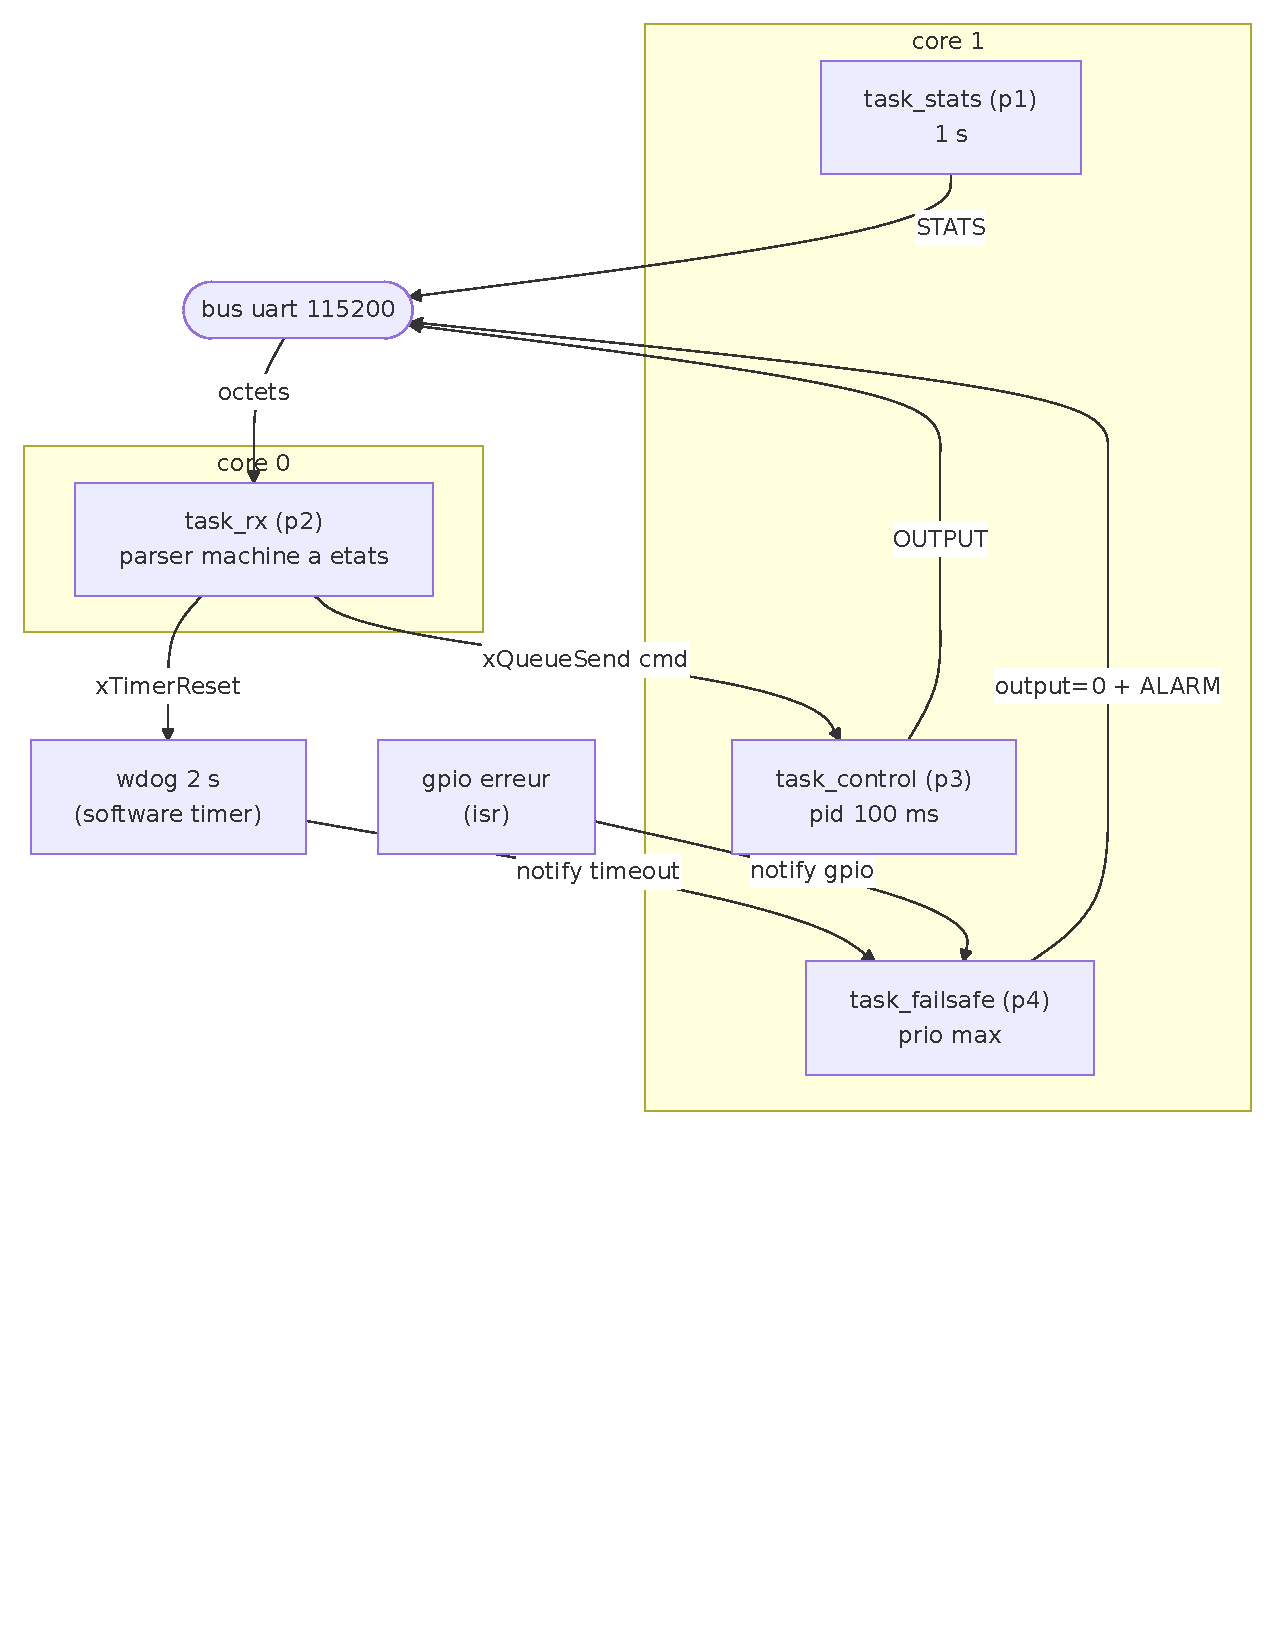
\includegraphics[width=0.95\textwidth]{archi.pdf}\\
    \small tâches, cœurs et flux d'événements
\end{center}

Événements : arrivée d'octets uart (rx décode, push queue, réarme le watchdog) ;
tick 100 ms (control dépile, calcule, émet en mode auto) ; tick 1 s (stats émet) ;
2 s sans trame valide (timer expire, notifie failsafe) ; front gpio d'erreur
(isr notifie failsafe) ; \texttt{mode\_set} (rx remet le mode et efface le flag
failsafe, reprise exigence 06).

\section{Justification des mécanismes FreeRTOS}

\begin{itemize}
    \item \textbf{queue} rx vers control : découple producteur et consommateur,
    lisse les rafales, envoi non bloquant (timeout 0) pour ne pas ralentir le parser.
    \item \textbf{mutex} sur l'émission uart : trois tâches émettent
    (control, stats, failsafe), sans protection deux écritures entrelaceraient
    leurs octets (interdit nf03). On prend un mutex et pas un sémaphore pour
    l'\textbf{héritage de priorité} : si stats (p1) tient le mutex et que failsafe
    (p4) le demande, stats est remontée à p4 le temps de libérer, pas d'inversion
    de priorité (nf04).
    \item \textbf{section critique / spinlock} pour les compteurs et l'état :
    accès de quelques cycles, sur dual core il faut un spinlock pour rester
    cohérent entre les cœurs, plus rapide qu'un mutex.
    \item \textbf{software timer} pour le watchdog rx : one-shot de 2 s réarmé à
    chaque trame valide, son callback notifie failsafe s'il expire. pas de tâche
    qui boucle.
    \item \textbf{task notification} pour réveiller failsafe : le plus rapide
    depuis une isr ou un callback, la valeur transporte la cause (gpio ou timeout).
    \item \textbf{vTaskDelayUntil} pour control et stats : période absolue sans
    dérive (un vTaskDelay accumulerait le temps de calcul et ferait du jitter).
\end{itemize}

\section{Charge cpu théorique}

Tick FreeRTOS réglé à 1000 Hz (1 ms) dans \texttt{sdkconfig.defaults} : à 100 Hz
la résolution serait de 10 ms, impossible de garantir un jitter sous 5 ms. Les
wcet ci-dessous sont des estimations (pas de mesure oscillo).

Core 1 : control (dépile + pid + trame output) estimé 200 us / 100 ms =
\textbf{0,2 \%} ; stats estimé 500 us/s = \textbf{0,05 \%} ; failsafe négligeable.
Total core 1 sous \textbf{1 \%}.

Core 0 : rx reçoit à 115200 bauds, soit 11520 octets/s, chaque octet passant dans
le parser (~0,5 us) plus le coût du driver, ce qui reste autour de \textbf{1 à
2 \%} même en flood continu.

Même sous surcharge uart maximale, le core 1 (la régulation) n'est donc quasiment
pas chargé et le pid garde son déterminisme.

\section{Priorité de l'uart par rapport au contrôle moteur}

Si on traitait l'uart en priorité haute, un flood retarderait le pid et la
période de 100 ms ne serait plus tenue. On fait l'inverse : \textbf{control
(prio 3) est au dessus de rx (prio 2)}, donc un cycle pid préempte le parser. Les
deux tâches sont en plus sur des cœurs différents, elles ne se disputent donc pas
le cpu. La réception n'est pas sacrifiée pour autant : la queue absorbe les
rafales, et la perte éventuelle sous flood extrême est comptée (dropped) sans
bloquer. La régulation prime, la réception se dégrade proprement.

\section{Choix des priorités et préemption}

Ordonnanceur préemptif à priorité fixe. L'ordre suit la criticité temps réel :
\textbf{failsafe (4)} la sécurité passe avant tout, dès qu'elle est notifiée elle
préempte n'importe quoi et force output=0 sous 5 ms sans attendre le prochain
cycle pid (l'isr gpio se limite à une notification) ; \textbf{control (3)} la
régulation, prioritaire sur tout sauf la sécurité ; \textbf{rx (2)} important mais
ne doit pas perturber control ; \textbf{stats (1)} aucune contrainte dure. La
préemption joue donc failsafe \textgreater{} control \textgreater{} rx
\textgreater{} stats, exactement l'ordre voulu.

\section{Monitoring et debug}

\begin{itemize}
    \item \textbf{trame stats (0x83)} sur le bus chaque seconde : rx valides, crc
    erreur, dropped, tx output, unknown (ids inconnus). l'outil pc suit l'ecu en direct.
    \item \textbf{log console} sur l'uart0 (séparé du bus sur uart2) : mode, flag
    failsafe, compteurs, \textbf{heap libre} (\texttt{esp\_get\_free\_heap\_size},
    détecte une fuite) et \textbf{jitter max} du pid (\texttt{jit\_max}, via
    \texttt{esp\_timer\_get\_time}).
    \item \textbf{led} sur le gpio 2 : allumée en failsafe, éteinte à la reprise,
    debug visuel sans console.
    \item séparer le bus binaire (uart2) des logs texte (uart0) évite de polluer
    les trames.
\end{itemize}

\section{Analyse de robustesse}

Le script de stress injecte : trames collées, fragmentées, crc faux, ids inconnus,
flood. La robustesse repose sur le parser, une machine à états
(start, len, data, crc) qui garde son état entre deux lectures uart.

\begin{itemize}
    \item \textbf{fragmentées} : on décode octet par octet en conservant l'état,
    une trame coupée reprend là où elle s'était arrêtée.
    \item \textbf{collées} : après une trame complète on repart à start, l'octet
    suivant est aussitôt le début de la trame d'après.
    \item \textbf{crc faux} : on recalcule le xor (len+type+payload), si ça ne
    colle pas on jette, on compte (crc++) et on resynchronise.
    \item \textbf{len incohérente} : len nul ou trop grand, on rejette et on
    repart à start, pas de débordement.
    \item \textbf{id inconnu} : trame valide mais type non géré, ignorée, unknown++
    (le crc était bon donc pas compté en erreur crc).
    \item \textbf{flood} : le parser tourne sur le core 0 sans toucher au pid
    (core 1), la queue absorbe et droppe en comptant si elle sature.
\end{itemize}

Les deux déclencheurs de failsafe sont indépendants : silence du pc (watchdog 2 s)
ou front gpio d'erreur (sous 5 ms grâce à la tâche prioritaire). Un \texttt{mode\_set}
auto relance ensuite.

\textbf{Tests.} D'abord un test unitaire de la couche protocole sur pc (construction
de trame, crc, même machine à états que le firmware), compilé avec
\texttt{-Wall -Wextra -Werror} : les six cas (trame propre, collées, fragmentée,
crc cassé, id inconnu) se comportent comme prévu. Ensuite le firmware complet
(esp-idf v5.4.4) sous \textbf{qemu xtensa}, le bus uart2 exposé sur un socket tcp,
avec le script de stress fourni : c'est le scénario complet rejoué de bout
en bout.

\begin{center}
    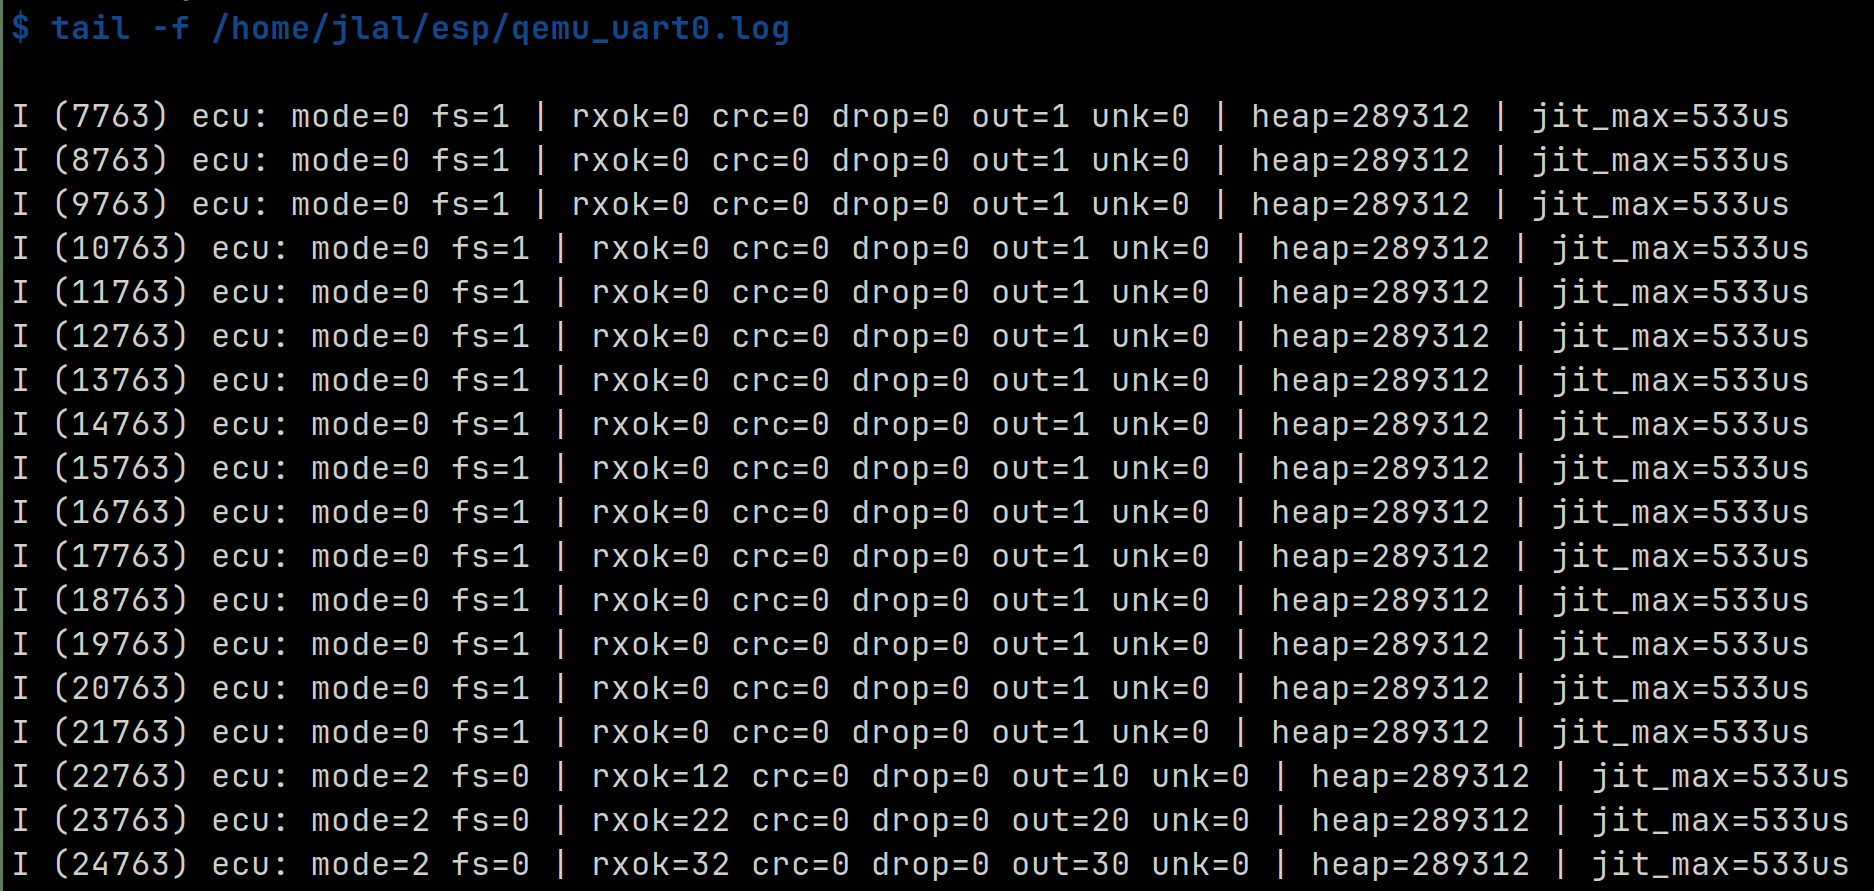
\includegraphics[width=0.95\textwidth]{qemu_counters.png}\\
    \small run qemu : passage en mode auto (\texttt{mode=2}), régulation qui
    démarre (\texttt{rxok}, \texttt{out} montent), \texttt{drop=0}. sous flood
    \texttt{unk} et \texttt{crc} montent (totaux \texttt{unk=50}, \texttt{crc=2}).
\end{center}

La trace confirme : régulation en mode auto, les 50 trames aléatoires comptées en
\texttt{unk=50} sans planter, les deux trames cassées en \texttt{crc=2},
\texttt{drop=0} sur tout le run (la queue n'a jamais débordé), failsafe au silence
(\texttt{fs=1}, \texttt{output=0}, alarme, le script affiche \texttt{verification
reussie}) et \texttt{heap} stable. La seule chose que qemu ne valide pas, c'est le
timing exact (pas cycle-accurate), donc on l'a mesuré sur carte.

\textbf{Validation sur cible.} Firmware flashé sur un ESP32-D0WD-V3 (dual core,
240 MHz). Boot ok, gpio configurés (led en sortie, entrée d'erreur en pullup sur
front descendant), et comme rien n'émet le watchdog déclenche le failsafe à 2,3 s
(\texttt{cause=1}). On a instrumenté \texttt{task\_control} avec
\texttt{esp\_timer\_get\_time} : à chaque cycle on mesure l'écart à la période de
100 ms et on garde le pire cas. Sur la carte \textbf{jit\_max plafonne à 179 us
(0,18 ms)}, largement sous les 5 ms demandés.

\begin{center}
    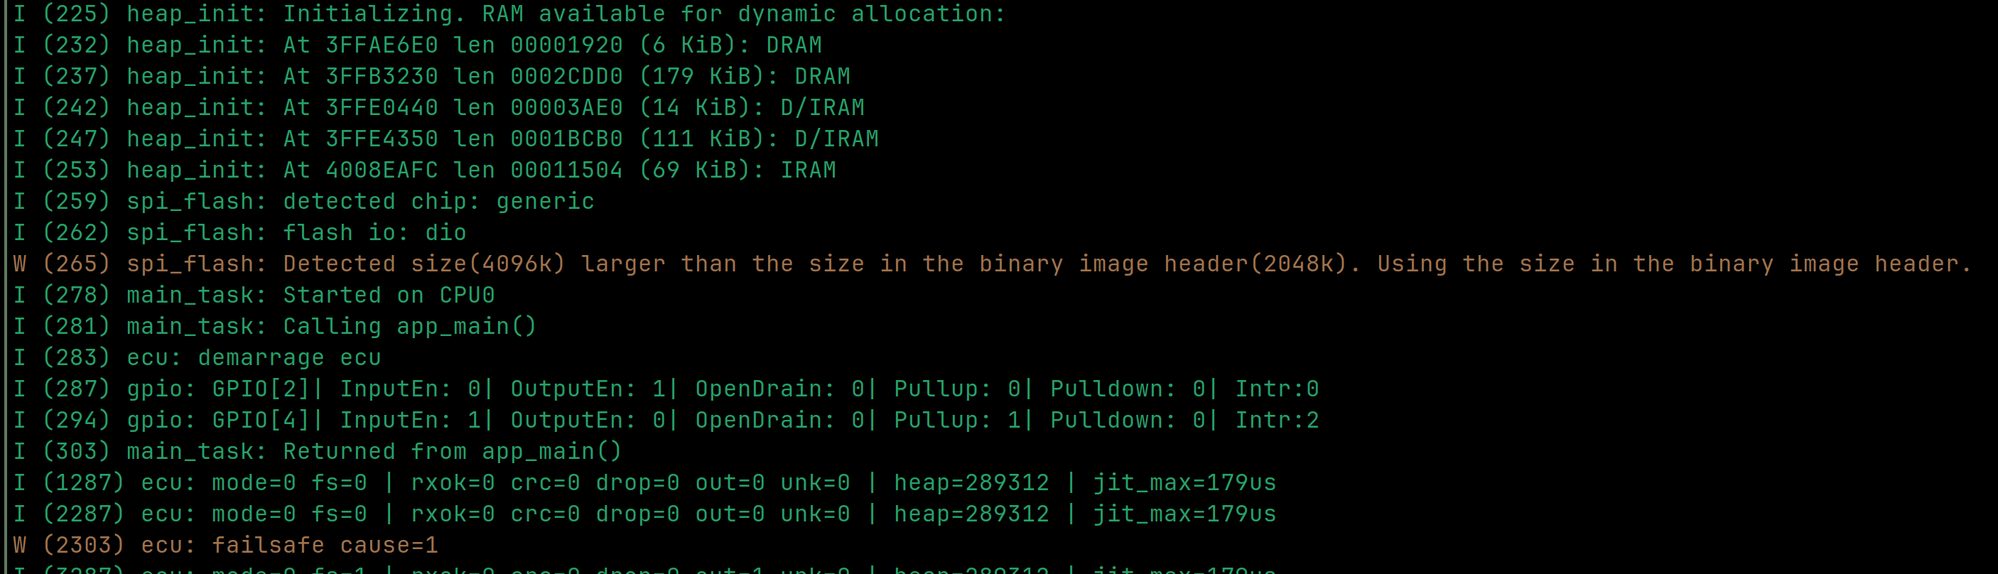
\includegraphics[width=0.95\textwidth]{hw_console.png}\\
    \small esp32 réel : démarrage, config gpio, télémétrie avec le jitter mesuré
    (\texttt{jit\_max=179us}) et failsafe watchdog (\texttt{cause=1})
\end{center}

\section{Limitations}

\begin{itemize}
    \item testé sous qemu (stress complet) et sur carte (boot, failsafe watchdog,
    jitter 0,18 ms). pas pu rejouer le \textbf{flood réel} sur la carte : le bus
    est sur uart2, il aurait fallu un second adaptateur usb-série sur les gpio
    16/17. le jitter sous forte charge externe reste à confirmer.
    \item \textbf{wcet et charge cpu} sont des estimations, à confirmer avec
    \texttt{vTaskGetRunTimeStats} et le high water mark.
    \item \textbf{coefficients pid} (kp=1, ki=0.1, kd=0.01) ceux fournis, pas
    réglés pour un vrai véhicule.
    \item pas de persistance : au reset on repart en mode off, compteurs à zéro.
\end{itemize}

\end{document}
